%!TEX program = xelatex

\documentclass[varwidth,convert]{BHCexam1_simple}
\usepackage{gensymb}
\usepackage{mathrsfs}
\usepackage{tikz,pgfplots,float} %绘图
\usepackage{tkz-euclide}
\usepackage{graphicx}
\usepackage{wrapfig}
\usepackage[english]{babel}
\usepackage{caption}
\usepackage{CJK}
\usepackage{enumitem}
\usetikzlibrary{calc,quotes,angles,babel,intersections,arrows,automata,positioning}

\pgfplotsset{compat=1.15}
\tikzset{ 
  right angle quadrant/.code={ 
   \pgfmathsetmacro\quadranta{{1,1,-1,-1}[#1-1]} % Arrays for selecting quadrant 
   \pgfmathsetmacro\quadrantb{{1,-1,-1,1}[#1-1]}}, 
  right angle quadrant=1, % Make sure it is set, even if not called explicitly 
  right angle length/.code={\def\rightanglelength{#1}}, % Length of symbol 
  right angle length=2ex, % Make sure it is set... 
  right angle symbol/.style n args={3}{ 
   insert path={ 
   let \p0 = ( $(#1)!(#3)!(#2)$ ) in % Intersection 
    let \p1 = ( $(\p0)!\quadranta*\rightanglelength!(#3)$ ), % Point on base line 
    \p2 = ( $(\p0)!\quadrantb*\rightanglelength!(#2)$ ) in % Point on perpendicular line 
    let \p3 = ( $(\p1)+(\p2)-(\p0)$ ) in % Corner point of symbol 
   (\p1) -- (\p3) -- (\p2) 
   } 
  } 
}

\setlength{\textwidth}{20cm}

\begin{document}

%%% -------- Anchor Start -------- %%%

如下图,已知在直角~$\triangle ABC$~中,~$\angle C=90\degree$,~$AC=7$,$BC=5$,
% \stk{}

\begin{enumerate}[label={(\arabic*)}]
\item 点到的距离为\stk 。
\item 在图中作出点到的距离。
\end{enumerate}
% \twoch{a}{b}{c}{d}
\hfill
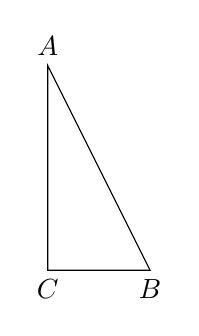
\begin{tikzpicture}[scale=1.3]
\coordinate [label=below:$C$] (C) at (0,0);
\coordinate [label=below:$B$] (B) at (1,0);
\coordinate [label=above:$A$] (A) at (0,2);
\draw (C) -- (B) -- (A) -- cycle;
\end{tikzpicture}

%%% -------- Anchor End ---------- %%%

\end{document}